\documentclass[10pt]{article}\usepackage[margin=.65in]{geometry}\usepackage[T1]{fontenc}\usepackage{graphicx}\setlength{\parindent}{0pt}\setlength{\parskip}{7pt}\sloppy\begin{document}{\large Component membership and root-size preservation}\par Thirteen declarations and six controls compiled. Nineteen separate named axiom readbacks passed; independent source-fidelity review is pending. These are bounded formal checks, not scientific measurements.\par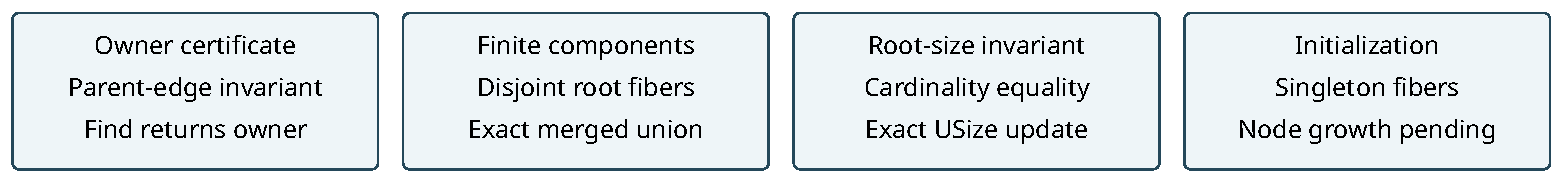
\includegraphics[width=\linewidth]{diagram.pdf}\par Construction. A component-owner certificate requires owner labels to be constant along parent edges and owner-fixed vertices to be exactly graph roots. The existing recursive GraphFind.Run preserves this certificate and returns the recorded owner. Combined with the established forest termination theorem, every vertex has a run reaching that owner. Thus the finite owner fibers identify the roots reached by the modeled find, rather than arbitrary labels.

Cardinalities. Fibers of distinct roots are disjoint. Attaching a child root to a parent root replaces the parent's fiber by the union of the two old fibers; other surviving root fibers remain unchanged. The root-size invariant records equality of each surviving root's stored USize value and fiber cardinality. It is preserved by find and by attachment with the previous exact-addition theorem and n$<$USize.size. The child's old size slot is retained but is no longer asserted to be a root size.

Initialization. The identity parent map and a fixed-length size array of ones satisfy both invariants. This includes the native one-node starting shape. Dynamic node insertion is still a separate obligation: this packet does not prove extension of the existing arrays and component map from n to n+1. The native word-to-field graph decoding must retain the preceding module bindings when these lemmas are composed into the full collector.

Controls. A three-vertex membership map has component cardinalities two and one. Both attachment orientations produce cardinality three at the surviving root, the old child fiber becomes empty, distinct fibers are disjoint, and a nonempty fiber is not disjoint from itself. These fixed logical controls are not a random sample. The geometric incoming relation, fixed-anchor collision return, allocation behavior and operation counters retain their separate proof obligations.

Verification and retained failures. Final modules and separate readback exited zero with unchanged bound source/toolchain/dependency files. The false theorem was rejected, as were empty, wrong-name and sorryAx inventories. Earlier induction-pattern, finite-set simplification and premature dependent-module attempts remain recorded. Imported compiled dependencies were reused, not independently rebuilt; before/after file hashes do not exclude transient edits. No new scientific run, runtime admission, measured cost or deadline change occurred.

Next review. Publish the exact sources and obtain separate review of owner certificates, find semantics, union membership and the root-only size invariant. Continue with dynamic node insertion and full native branch composition, preserving all current assumptions until discharged. The graph shows proof dependencies and the remaining insertion boundary; no comparative performance claim is made.
\end{document}